%
% This is the LaTeX template file for lecture notes for CS294-8,
% Computational Biology for Computer Scientists.  When preparing 
% LaTeX notes for this class, please use this template.
%
% To familiarize yourself with this template, the body contains
% some examples of its use.  Look them over.  Then you can
% run LaTeX on this file.  After you have LaTeXed this file then
% you can look over the result either by printing it out with
% dvips or using xdvi.
%
% This template is based on the template for Prof. Sinclair's CS 270.

\documentclass[11pt, twosides]{article}
\usepackage[utf8]{inputenc}
\usepackage{graphicx}
\usepackage{graphics}
\usepackage{amsmath}
\usepackage{amsfonts}
\usepackage{amssymb}
\usepackage{amsthm}
\usepackage{xcolor}
\setlength{\oddsidemargin}{0.25 in}
\setlength{\evensidemargin}{-0.25 in}
\setlength{\topmargin}{-0.6 in}
\setlength{\textwidth}{6.5 in}
\setlength{\textheight}{8.5 in}
\setlength{\headsep}{0.75 in}
\setlength{\parindent}{0 in}
\setlength{\parskip}{0.1 in}

%
% The following commands set up the lecnum (lecture number)
% counter and make various numbering schemes work relative
% to the lecture number.
%
\newcounter{lecnum}
\renewcommand{\thepage}{\thelecnum-\arabic{page}}
\renewcommand{\thesection}{\thelecnum.\arabic{section}}
\renewcommand{\theequation}{\thelecnum.\arabic{equation}}
\renewcommand{\thefigure}{\thelecnum.\arabic{figure}}
\renewcommand{\thetable}{\thelecnum.\arabic{table}}

%
% The following macro is used to generate the header.
%
\newcommand{\lecture}[4]{
%   \pagestyle{myheadings}
   \thispagestyle{plain}
   \newpage
   \setcounter{lecnum}{#1}
   \setcounter{page}{1}
   \noindent
   \begin{center}
   \framebox{
      \vbox{\vspace{2mm}
    \hbox to 6.28in { {\bf CS 419M Introduction to Machine Learning
                        \hfill Spring 2021-22} }
       \vspace{4mm}
       \hbox to 6.28in { {\Large \hfill Lecture #1: #2  \hfill} }
       \vspace{2mm}
       \hbox to 6.28in { {\it Lecturer: #3 \hfill Scribe: #4} }
      \vspace{2mm}}
   }
   \end{center}
   \markboth{Lecture #1: #2}{Lecture #1: #2}
}

%
% Convention for citations is authors' initials followed by the year.
% For example, to cite a paper by Leighton and Maggs you would type
% \cite{LM89}, and to cite a paper by Strassen you would type \cite{S69}.
% (To avoid bibliography problems, for now we redefine the \cite command.)
% Also commands that create a suitable format for the reference list.
% \renewcommand{\cite}[1]{[#1]}
% \def\beginrefs{\begin{list}%
%         {[\arabic{equation}]}{\usecounter{equation}
%          \setlength{\leftmargin}{2.0truecm}\setlength{\labelsep}{0.4truecm}%
%          \setlength{\labelwidth}{1.6truecm}}}
% \def\endrefs{\end{list}}
% \def\bibentry#1{\item[\hbox{[#1]}]}

%Use this command for a figure; it puts a figure in wherever you want it.
%usage: \fig{NUMBER}{SPACE-IN-INCHES}{CAPTION}
% \newcommand{\fig}[3]{
% 			\vspace{#2}
% 			\begin{center}
% 			Figure \thelecnum.#1:~#3
% 			\end{center}
% 	}
% Use these for theorems, lemmas, proofs, etc.
\newtheorem{theorem}{Theorem}[lecnum]
\newtheorem{lemma}[theorem]{Lemma}
\newtheorem{proposition}[theorem]{Proposition}
\newtheorem{claim}[theorem]{Claim}
\newtheorem{corollary}[theorem]{Corollary}
\newtheorem{definition}[theorem]{Definition}
% \newenvironment{proof}{{\bf Proof:}}{\hfill\rule{2mm}{2mm}}

% **** IF YOU WANT TO DEFINE ADDITIONAL MACROS FOR YOURSELF, PUT THEM HERE:

\begin{document}
%FILL IN THE RIGHT INFO.
%\lecture{**LECTURE-NUMBER**}{**DATE**}{**LECTURER**}{**SCRIBE**}
\lecture{7}{Binary Classification}{Abir De}{Alakh Agrawal, Devanshu Sarraf, Aditya Kudre}
%\lecture{x}{Title}{Abir De}{Group y}

\section{Classification}
We will study the following under classification:
\begin{enumerate}
    \item What is a classification task?
    \item What are the classification models?
    \item Depth of support vector machines
\end{enumerate}

\subsection{Binary Classification Problem}
Suppose we are given a set of points and we need to classify them as \textbf{Red} or \textbf{Blue} based on their x coordinate. \\*[-0.1cm]

\begin{figure}[hpt!]
	\centering
  %  \noindent
%	\begin{flushright}
 	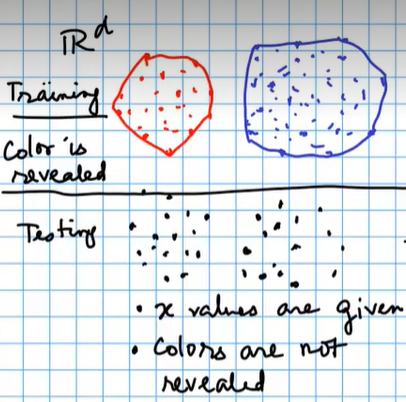
\includegraphics[width=0.35\linewidth,right]{task.PNG} % Replace 
 %	\end{flushright}
 	%'myplot.png' with the filename of your image file. Only PNG, JPG and PDF images are allowed. This image file should be in the same folder.
%	\caption{Plot for Axial Stress($\sigma_x$(MPa)) vs distance from beam mid-depth(y(mm)) at the quarter-span of the beam}
\end{figure}
\vspace{0.3cm}
\textbf{Input:} D = \{$(x_i, y_i) \hspace{0.1cm} \big| \hspace{0.1cm} y_i \in \{ -1, +1 \} $\}. 
\textbf{Find:  } $m(x) \xrightarrow{} y$

Let $P_m(y \vert x) = \frac{1}{1+e^{-w^\top x y}} \Rightarrow \max\limits_{w} \prod P_m(y_i \vert x_i) \xrightarrow$ $\max\limits_{w} \sum log(P_m(y_i \vert x_i)) \xrightarrow$ $\min\limits_{w} \sum log(1+e^{-w^\top x y})$


\newpage
\subsection{Trying out a Linear Model}

Simplifying this problem as: \\
if, $w^\top x + b > 0 \Rightarrow y=+1$ \\
else, $w^\top x + b < 0 \Rightarrow y=-1$ \\

This can cause a problem if two points are too close, hence let's take a small $\Delta$ instead of $0$ \\
if, $w^\top x + b > \Delta \Rightarrow y=+1$ \\
else, $w^\top x + b < -\Delta \Rightarrow y=-1$ \\*[0.5cm]
This will lead to a problem while classifying the points around the margin and cannot be resolved for however small $\Delta$.

The problem is that when we have points close to the margin, it may be possible that these points are not classified at all as we have a finite non zero $\Delta$.

We can ignore the overlapping points,\\
Let ${I}^+ = \{ i \mid y_i = 1 \}$, ${I}^- = \{ i \mid y_i = -1 \}$,  ${S}^+ \in {I}^+$,${S}^- \in{I}^-$ such that $|{S^+} \cup {S^-}| = n $,
\begin{equation*}
    \min_{\zeta_i} { f(w) - \left( \sum_{i \in S^+} \mathbb{I}\left( w^Tx_i + b \ge \Delta \right) + \sum_{i \in S^-} \mathbb{I} \left( w^Tx_i + b \le \Delta \right) \right)}
\end{equation*}


\subsection{A possible solution}

We can have an additional loss function along with a usual convex loss function like mean squared error loss that would solve the issue of the above rare case.\\

This loss function will ensure that the number of points that are not classified or mis-classified is kept to a minimum number.\\

Thus, we have the following optimization problem:\\

$min_{w, b, S, S^{+}\bigcup S^{-} = S} [f(w, b) - \Sigma_{i \in S^+}I(w^Tx_i + b > \Delta, y_i = 1) - \Sigma_{i \in S^-}I(w^Tx_i + b < -\Delta, y_i = -1)]$\\

Here, $f(w, b)$ is our usual loss function while $I(condition)$ is the indicator function and $I(condition) = 1$ if the $condition$ is true else $I(condition) = 0$\\

Alternatively, we can also have the below optimization problem which involves a slightly different version of our additional loss function:\\

$min_{w, b, S, S^{+}\bigcup S^{-} = S} [f(w, b) + \Sigma_{i \in S^+}I(w^Tx_i + b > \Delta, y_i = -1) + \Sigma_{i \in S^-}I(w^Tx_i + b < -\Delta, y_i = 1)]$\\
%\newpage
\subsection{Another possible solution}

We could instead modify the model as follows:\\

$\forall y_i = 1, w^Tx_i + b > \Delta - \xi_i$\\
$\forall y_i = -1, w^Tx_i + b < -\Delta + \xi_i$\\

Here, $\xi_i$ is also a parameter that is to be trained and $\xi_i > 0$ $\forall$ $i \in D$. Then, we have the following optimization problem:\\

$min_{w, b, \xi_i} [f(w, b) + \Sigma_{i \in D}\xi_i]$ such that $y_i(w^Tx + b) > \Delta - \xi_i$ $\forall$ $i \in D$


%\begin{flushleft}
%Q. \textbf{What is the underlying thesis/concept behind the hope that it will be possible to train the model $m_\theta$ to get an accurate output?}\\

%Ans. \color{blue}
%\textbf{The law of large numbers}
%\end{flushleft}

%\subsection{The Law of Large Numbers and Central Limit Theorem}
%Suppose that we have $N$ samples $X_i \sim f(\cdot), \:\:\: i = 1, \hdots, N$ drawn from an unknown distribution. Most of the times, the goal of machine learning is to estimate the distribution $f$ or its properties. For example, in the task of generating images (GAN, VAE etc), the objective of the machine learning model is to identify the underlying distribution of the data samples. Being able to learn the underlying distribution is important even for tasks like housing price prediction, image classification etc because if a test sample is sampled from a different distribution is given to the model, the model will likely fail and give incorrect results. 
%\begin{flushleft}
%Q. \textbf{What is the least that can be found about $f$ using $X_1, \hdots, X_N$?}\\

%Ans. \color{blue} Central Limit Theorem states that as long as $N$ is large, the $$\mathbb{E}_{X \sim f(\cdot)}[X] = \frac{\sum X_i}{N}$$
%The Law of Large Numbers further states that
%$$\mathbb{E}_{X \sim f(\cdot)}[X] \xrightarrow{}\frac{\sum X_i}{N}$$
%as $N \xrightarrow{} \infty$. Moreover, the random variable $Z_N = \frac{\sum X_i}{N}$ follows the normal distribution $\mathcal{N}(\mathbb{E}[X], \sigma^2)$
%with $\sigma^2 \propto \frac{1}{N}$ with
%$$\lim \limits_{N \xrightarrow{}\infty}\mathbb{E}[Z_N] = %\mathbb{E}[X]$$
%\end{flushleft}
%\begin{flushleft}
%Q. \textbf{What else do we need to completely characterize $f$?}\\

%Ans. \color{blue} \textbf{We need the higher order moments!} Using %these the moment generating function can be obtained.
%\end{flushleft}

%\definition{The moment generating function (MGF) $F(s)$ for a random variable $X$ is defined as the Laplace Transform of the probability density function (PDF) $f(x)$. The inverse Laplace Transform of MGF will give the PDF.
%$$F(s) = \int \limits_{-\infty}^\infty e^{-sx}\, f(x)\, dx$$
%$$f(x) = \int \limits_{-\infty}^\infty e^{sx}\, F(s)\, ds$$}

%\proposition{Using only the moments, the MGF can be determined.}
%\begin{proof}
%\begin{eqnarray*}
%F(s) &=& \int \limits_{-\infty}^\infty e^{-sx}\, f(x)\, dx\\
%&=& \int \limits_{-\infty}^\infty \sum \limits_{k = 0}^{\infty} %\frac{(-s)^k\, x^k}{k!}\, f(x)\, dx\\
%&=& \sum \limits_{k = 0}^{\infty} \frac{(-s)^k}{k!}\, \mathbb{E}[X^k]
%\end{eqnarray*}
%\begin{flushleft}
%Note: The discussion about the region of convergence of the Laplace transform is out of the scope of this course.
%\end{flushleft}
%\end{proof}

%\proposition{
%Using just the $N$ samples $X_i \sim f(\cdot), \:\:\: i = 1, \hdots, N$, the PDF $f$ can be estimated using the Law of Large Numbers.
%%%%%%%%%%%%}
%%%%%%%%%%%\begin{proof}
%%%%%%%%%%This can be proved as follows:
%%%%%%%%%\begin{enumerate}
%%%%%%%%    \item All moments $\mathbb{E}[X^k]$ can be estimated by invoking the Law of Large Numbers
%%%%%%%    \item The MGF can be found by invoking the Claim 1.2 above.
 %%%%%%   \item $f$ can be estimated by taking the inverse Laplace Transform of the MGF
%%%%%\end{enumerate}
%%%%\end{proof}

%%%\subsection{Practice Problems}
%%\normalfont
%\begin{enumerate}
 %%%%%%%%%%%%   \item  A fair coin is tossed 5 times. Find  $\mathbb{P}(\#H > \# T)$\\
 %%%%%%%%%%%   \color{blue}It is easy to see that as 5 is odd, there is not possibility of %%%%%%%%%%$\#H = \#T$. Hence $\mathbb{P}(\#H > \# T) = 1/2$
 %%%%%%%%%%   \color{black}
 %%%%%%%%%   \item $X \sim f(\cdot), Y \sim g(\cdot)$. Then $Z = X+Y \sim \:?$\\
%%%%%%%%    \color{blue} \begin{eqnarray*}
 %%%%%%%   \mathbb{P}(Z \leq z) &=& \mathbb{P}(X+Y \leq z)\\
  %%%%%%                      &=& \int \limits_{-\infty}^\infty \int \limits_{-\infty}^{z-x}f(x) \, g(y) \, dx\,dy\\
  %%%%%                      &=& \int \limits_{-\infty}^\infty f(x)\, G(z-x) \, dx
  %%%%  \end{eqnarray*}
  %%%  On differentiating, we get
 %%   $$f_Z(z) = \int \limits_{-\infty}^\infty f(x) g(z-x)\,dx = (f * g)(z)$$
%\end{enumerate}
%%%%%%%%%%%%%%%\section{Linear Algebra}
%%%%%%%%%%%%%%Solve the following problems:
%%%%%%%%%%%%%\begin{enumerate}
 %%%%%%%%%%%%   \item For two square matrices $A, B$of size $n\times n$ if $AB = BA$ for all B, then show that $A = cI_n$ for some $c \in \mathbb{R}$\\
 %%%%%%%%%%%   \color{blue}
 %%%%%%%%%%   Pick $B$ to be a diagonal matrix with pair-wise distinct elements. Then it can be shown that $A$ is also a diagonal matrix. Now pick $B$ to be a matrix with all ones, i.e. $B = [1]_{ij}$. As $A$ is diagonal, $AB=BA$ implies all diagonal entries of $A$ are equal i.e., $A = cI_n$ for some $c \in \mathbb{R}$
  %%%%%%%%%%  \color{black}
 %%%%%%%%%   \item If $x^\top A x = 0\:\: \forall x \in \mathbb{R}^n$ then show that $A$ is skew-symmetric.\\
 %%%%%%%%   \color{blue}
 %%%%%%%   On differentiating the above equation we get
 %%%%%%   $$(A + A^\top)x = 0 \:\: \forall x \in \mathbb{R}^n$$
 %%%%%   This implies $A = -A^\top$
 %%%%   \color{black}
 %%%   \item Show that $\text{rank}(AB) \leq \text{rank}(A)$\\
%%    \color{blue} Each column of $AB$ can be viewed as a linear combination of columns of $A$. Hence, if the dimension of column space of $A$ is $r$, the dimension of column space of $AB$ cannot be more than $r$. In other words,
%    $\text{rank}(AB) \leq \text{rank}(A)$
 %%%%%%%%%%%%   \color{black} 
%%%%%%%%%%%    \item Suppose you have a uniform sampler which samples uniformly from $[0, 1]$. Propose an algorithm which uses this uniform sampler to generate samples from any given distribution.\\
 %%%%%%%%%%   \color{blue}
 %%%%%%%%%   Suppose we have a uniform random variable $U \sim \text{Uniform}([0, 1])$. We need to find a function $g$ such that the PDF of the random variable $g(U)$ will be same as that of the given distribution, say $f$. That is $g(U) \sim f$. Which is same as
  %%%%%%%%  \begin{eqnarray*}
 %%%%%%%   \mathbb{P}(g(U) \leq x) &=& \mathbb{P}(U \leq g^{-1}(x))\\
 %%%%%%   \implies \int \limits_{-\infty}^x f(x) \, dx &=& \int \limits_{-\infty}^{g^{-1}(x)} 1 \, du\\
 %%%%%   \implies F(x) &=& g^{-1}(x)\\
 %%%%   \implies g &=& F^{-1}
 %%%   \end{eqnarray*}
 %%   \color{black}
%\end{enumerate}
\section{Group Details and Individual Contribution}
% Fill this part
\textbf{Alakh Agrawal (200040018):} Section 7.1, 7.1.1, 7.1.2 (Binary Classification Problem, Trying out a Linear Model)\\
\textbf{Devanshu Saraf (200040042):} Section 7.1.2 (Binary Classification Problem, Trying out a Linear Model)\\
\textbf{Aditya Kudre (200070039):} Section 7.1.3, 7.1.4 (A possible solution, Another possible solution)
\end{document}





